\documentclass[aspectratio=1610]{beamer}

\usetheme[1610]{ZBH}
\usepackage{graphicx}
\usepackage{algorithm2e}
\usepackage{numprint}

\author{Florian Markowsky}
\title{Efficient storage of genome data}
\date{\today}

\begin{document}

\begin{frame}

\titlepage
\end{frame}

\begin{frame}
	\frametitle{Outline}
	\tableofcontents
\end{frame}

\section{Introduction}

\begin{frame}{Genome size}
  Problem: 
  \begin{itemize}
    \item Genomes are large: $10^5$ to $10^{10}$ BP
      %10^4: \alpha-Phage, 10^10: Teichmolch
    \item New sequencing technologies allow fast and cheap sequencing
      %first human genome draft: 10 years, 400 Mill$, now: 1 week, 10k$, massive paralelization
      %"1000 genomes project" and similar
      %sequencing of own genome affordable -> personalized medicine
    \item Genome data grows faster than processing power (Moore's Law)
      %Moores Law: number of transistors on integrated circuits doubles approx. every two years
        %dagegen: genomdaten ca. verzehnfachen/Jahr
      %-> storage budgets have to increase
    %\item Sequence search scales at least linear with database size
      %de facto: slows down exponentially every year
  \end{itemize}%TODO columns?!-< grafik größer
      \begin{figure}
        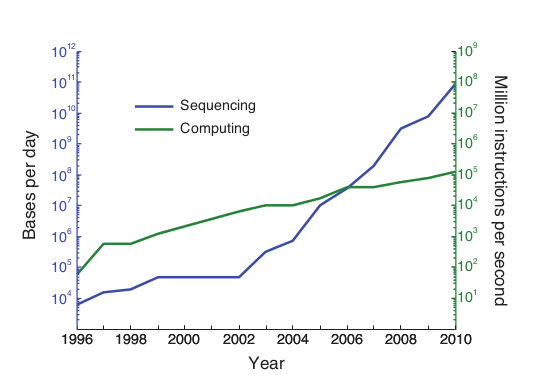
\includegraphics[height=0.3\textwidth]{img/Moorevsgen.png}
      \end{figure}
\end{frame}

\begin{frame}{Genome size}
  But:
  \begin{itemize}
    \item Single genome almost incompressible
      %but: in most cases, many have to be stored -> databases
    \item Highly similar in same species (human: $~1\%$ difference)
      %of 3gb, only 1% (=30 MB have to be stored if you have reference genome
    \item $\rightarrow$ if examining genome collections, only differences have to be stored
  \end{itemize}
  \vspace{0.5cm}
  Demands:
  \begin{itemize}
    \item Reduce file size as much as possible
    \item Optional:
      \begin{itemize}
        \item Fast compression
        \item Random access/partly decompression
      \end{itemize}
  \end{itemize}
\end{frame}

%usual compression techniques like LZ77: sliding window, compress by finding repeats in window) are not
%fit to deal with so long repeats (multi-gigabyte buffer would be necessary)

\section{State of research: different compression techniques}

\begin{frame}{Different Approaches}
  \begin{itemize}
    \item Reference based compression (Fritz, Leinonen, Chochrain \emph{et al. } 2011)
    \item Iterative dictionary for large DNA datasets (Kuruppu \emph{et al. } 2011)
    \item Robust relative compression with random access (Deorowicz, Grabowski 2011)
  \end{itemize}
\end{frame}

\subsection{Reference-based read compression}
\begin{frame}{Reference-based read compression - Algorithm}
  \begin{itemize}
    \item Stores short sequence reads
      %biggest amount of sequencing data emerges from next-generation sequencing techniques
    \item Alignment of reads to reference sequence
    \item Store position of reads, strand, Indel information
    \item Postitions relatively stored als Golomb-codes
      %if data is geometric distributed, golomb code is as efficient as Huffman, but needs less memory
  \end{itemize}
\end{frame}

\begin{frame}[plain]{Listen}
\vfill
\begin{center}
  \begin{figure}
    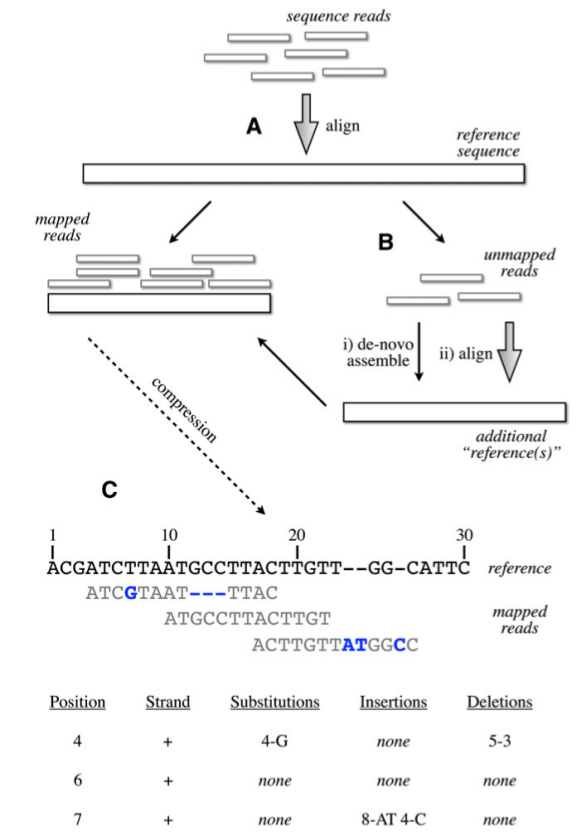
\includegraphics[height=0.6\textwidth]{img/ReadCompressionSchematic.png}
  \end{figure}
  \vfill
\end{center}
\vfill
\end{frame}

\begin{frame}{Reference-based read compression - Discussion}
  Problem: what to do with unaligned reads?
  \begin{itemize}
    \item Discard: loss of information
    \item Keep: high storage cost $\rightarrow$ other compression technique?
    %unmapped reads problem: can not be aligned
    %->pool unmapped reads, assemble to additional "reference sequence" (deBruijn)
    %but: not 
  \end{itemize}
  %TODO random access?
  \vspace*{0.5cm}
  Compression Results:\\
  \begin{tabular}{c|ccc}
    & reference based & raw FASTA & bzip2 \\
    \hline
    human genome & $0.41$ bpb & $11.45$ bpb & $1.84$ bpb \\
bacterial genome & $0.19$ bpb & $12.27$ bpb & $1.66$ bpb \\
  \end{tabular}
  \vspace*{0.5cm}\\
  $\rightarrow$ $10$- to $30$-fold better compression than standard approaches
\end{frame}


\subsection{Iterative dictionary construction: COMRAD}
\begin{frame}{COMRAD - Algorithm}%SEQUENZEN WERDEN KOMPRIMIERT, keine reads
  Dictionary construction by identifying repeated substrings in large DNA datasets %multiple passes over data
     \\ $\rightarrow$ works best on highly redundant datasets\\
      %gramar-based compression -> finding smallest gramar NP hard -> greedy
      In each iteration:
  \begin{itemize}
    \item Modify frequency-dictionary
    \begin{itemize}
      \item Count frequences of substrings 
    \end{itemize}
  \item Substitiution
    \begin{itemize}
      \item Substitute all new dictionary entries for new nonterminals
        %substitution is greedy
    \end{itemize}
    %two passes in each iteration
    %Number of iterations grows with size of data: +1/+2 it. pro decimal order of magnitude
    %example: Influenza-Dataset: 11 Iterations
  \item result iteration $k$: Dictionary $D_k$, Alphabet $\Sigma _k$, set $S_k$ of compressed sequences
  \end{itemize}
  final compression: Huffman
\end{frame}

\begin{frame}[plain]{Listen}
\vfill
\begin{center}
  \begin{figure}
    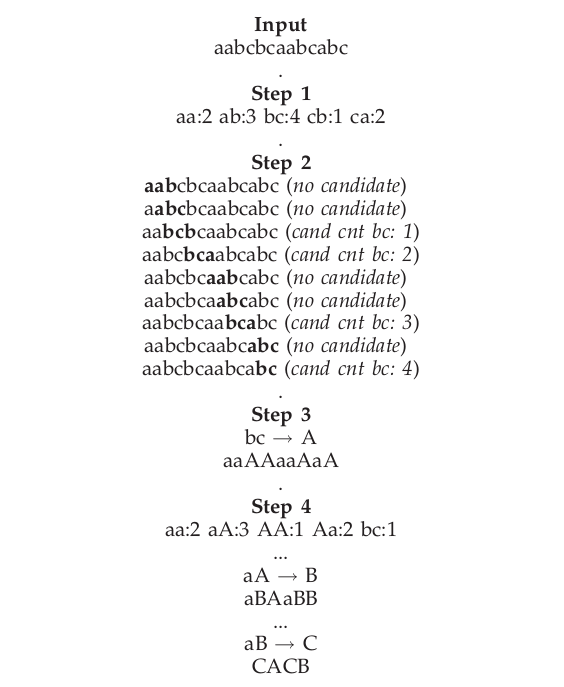
\includegraphics[height=0.6\textwidth]{img/Comrad.png}
    %Parameters: length L of substrings for first iteration (default: 16), 
    %frequency F(default:4): when to take words in dictionary
    %in consecutive runs, only sequences with nonterminal symbols must be considered 
    %(in certain patterns)
  \end{figure}
\end{center}
\vfill
\end{frame}

\begin{frame}{COMRAD -  Discussion}
  \begin{itemize}
      %slow encoding: frequence count: (N), substitution O(n log n)
    \item Provides random access and single sequence decompression
    \item Efficient on large dataset with many/long repeats
    \item Nearly no effect on small datasets with short repeats: disproportionately large codebook
  \end{itemize}
  \begin{itemize}
      %bpb = bits per base
    \item Influenza genomes $113$ MB ($1.97$ bpb) to $6$ MB ($0.43$ bpb)
    \begin{itemize}
      \item time for compression: about $0.03$h $\rightarrow$ $1.04$ MB/s
    \end{itemize}
      %time: 0.03h
    \item Yeast genomes $485.87$ MB ($2.19$ bpb) to $15.29$ MB ($0.25$ bpb)
    \begin{itemize}
      \item time for compression: about $0.19$h $\rightarrow$ $0.71$ MB/s
    \end{itemize}
      %time: 0.19
    \item 4 human genomes \numprint{12066.06} MB ($2.18$ bpb) to \numprint{2176.06}MB ($1.44$ bpb)
    \begin{itemize}
      \item time for compression: about $8$h $\rightarrow$ $0.42$ MB/s
    \end{itemize}
    %problem: codebook very large -> better when compressing bigger number of genomes:
    %   artificial generated human dna compressed to 0.07bpb (31.41gb to 0.29gb)
  \end{itemize}
\end{frame}

\subsection{Robust relative compression with random access}%TODO präziser ausführen?
\begin{frame}{Robust relative compression with random access - Algorithm}
  \begin{itemize}
    \item Input sequence is parsed in sequence of matches and literals 
    \item Hash array used to find matches
    %in contrast to suffix array (RLZ-opt): faster compression, less memory
    \item Lookahead buffer %match at $i+1$ longer than match at $i$? size changes dynamically
      %BUT shorter matches may be prefered if offset encoding is cheaper
      %also: penalty for mismatches
    \item Stores matches as pair of reference offset and match length\\ $\rightarrow$ Huffman
      %offsets encoded as differences between seq. pos in current genome and matched-to position in ref. genome
    \item Literals and reference sequence $\rightarrow$ Huffman%TODO nachlesen
  \end{itemize}
\end{frame}

\begin{frame}{Robust relative compression with random access - Discussion}
  \begin{itemize}
      %encoding way faster than COMRAD
    \item Allows random access to parts of compressed sequences due to blockwise coding
    \item 39 yeast genomes: $493.98$ MB compressed to $6.88$ MB, $33.15$ MB/s
  \item 70 human genomes: \numprint{218 961.98} MB compressed to \numprint{1 201.15}MB, 146.16 MB/s
  \end{itemize}
\end{frame}

\section{Genome ReSequencing tool}
\begin{frame}{Genome ReSequencing tool}
  GRS Algorithm computes compressed difference files 
  \begin{itemize}
    \item calculate varied sequence percentage $\delta$ for each chromosome based on a reference sequence
    \item if $\delta<0.03$
      \begin{itemize}
        \item compute different sequence file
      \end{itemize}
    \item if $0.03<\delta<0.1$
      %diesen schritt durchführen, wenn chromosome nicht ähnlich genug sind (kompression wäre ineffizient)
      %also: chromosom zerschneiden, neu gegen chromosom alignieren
      \begin{itemize}
        \item cut chromosome into $n$ pieces
        \item calculate each $\delta_i$
        \item find position with minimal $\Sigma \delta_i$
        \item compress each piece
      \end{itemize}
    \item if $\delta>0.1$: Data not suitable
  \end{itemize}
\end{frame}

\begin{frame}{Genome ReSequencing tool}
  \begin{columns}
  \begin{column}{6cm}
    \begin{itemize}
      \item find longest common local nucleotide sequences%TODO erklären, supplement
      \item example: gaNGCTA and gNGTNA
    \end{itemize}
  \end{column}
  \begin{column}{6cm}
    \begin{figure}
      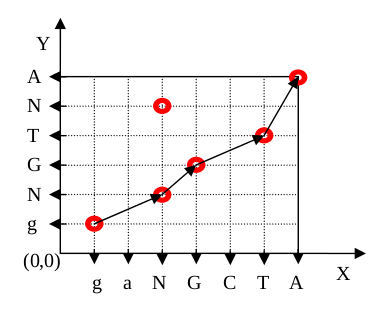
\includegraphics[height=0.6\textwidth]{img/WaZhComSub.png}
    \end{figure}
  \end{column}
  \end{columns}
\end{frame}

\begin{frame}{Genome ReSequencing tool}
  \begin{columns}
  \begin{column}{6cm}
    \begin{itemize}
      \item method to compute difference file similar to UNIX diff program
      \item process diff file to reduce size
      \item encode using Huffman
    \end{itemize}
  \end{column}
  \begin{column}{6cm}
    \begin{figure}
      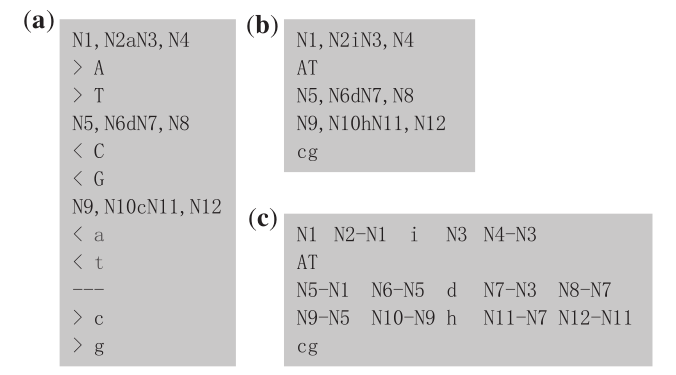
\includegraphics[height=0.6\textwidth]{img/WaZh2.png}
      %a. raw changes generated by diff
      %b. stripped of redundant information: does not matter WHAT was deleted
      %   bei ersetzungen egal was ersetzt wurde
      %c. relative Positionsangaben
    \end{figure}
  \end{column}
  \end{columns}
\end{frame}

\begin{frame}[plain]{Listen}
\vfill
\begin{center}
  \begin{figure}
    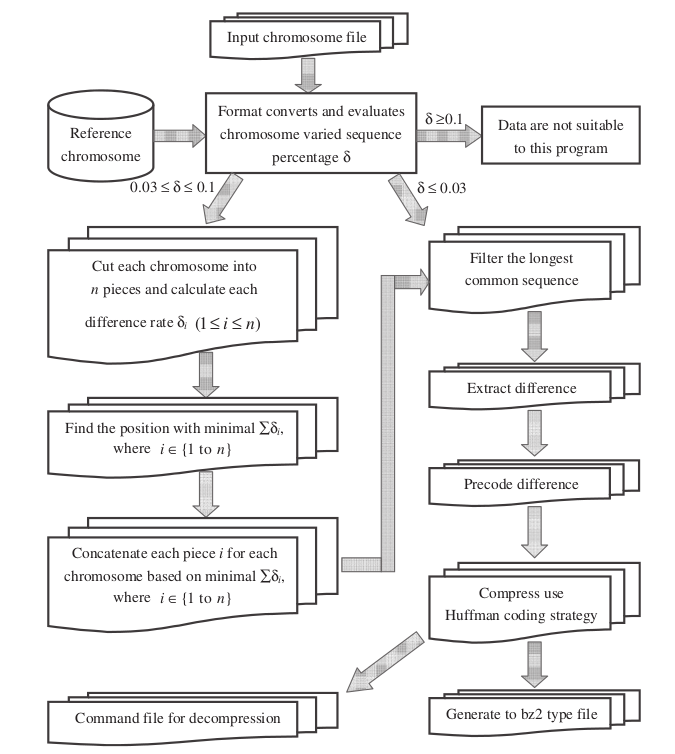
\includegraphics[height=0.7\textwidth]{img/WaZh.png}
  \end{figure}
  \end{center}
\end{frame}

\begin{frame}{Genome ReSequencing tool - Discussion}
  \begin{itemize}
    \item Allows encoding without knowledge of reference SNPs map
      %the other presented techniques dont need them, too
    \item Rice genomes: $361$ MB compressed to $4.4$ MB, $0.26$ MB/s
    \item Human genome: \numprint{2986.8} MB compressed to $18.8$ MB, $1.81$ MB/s
  \end{itemize}
  \begin{itemize}
    \item No random access
  \end{itemize}
\end{frame}

\section{What is to come...}
\begin{frame}{Future development}
  Presented Algorithms:
  \begin{itemize}
  \item  can compress effectively
  \item  are efficient enough to store many genomes on available disk space
\end{itemize}
but...
\begin{itemize}
  \item  Decompression necesarry for computation
  \item  Aim: algorithms computing on compressed data
    %many noncompressive algorithms will just not work on Terabyte of sequencing data
  \item  Next slides: a compressive BLAST algorithm is presented
    %Compression Accelerated BLAST
    %BLAST/BLAST principle is widely used -> improved blast would speed up many existant programs/tools
  \end{itemize}
\end{frame}

\begin{frame}{CaBlast - Algorithm}
  \begin{itemize}
    \item  Preprocession: compression of input data
      \begin{itemize}
        \item fill unique database with first occurances of substrings
        \item store repeats as pointers to subsequence from unique occurrence
      \end{itemize}
    \item CaBLAST:
      \begin{itemize}
        \item perform coarse BLAST Search on unique database \\
          $\rightarrow$follow pointers to repeats of hits
        \item perform fine BLAST Search on coarse-hits and decompressed repeats
      \end{itemize}
  \end{itemize}
\end{frame}

\begin{frame}[plain]{Listen}
\vfill
\begin{center}
  \begin{figure}
    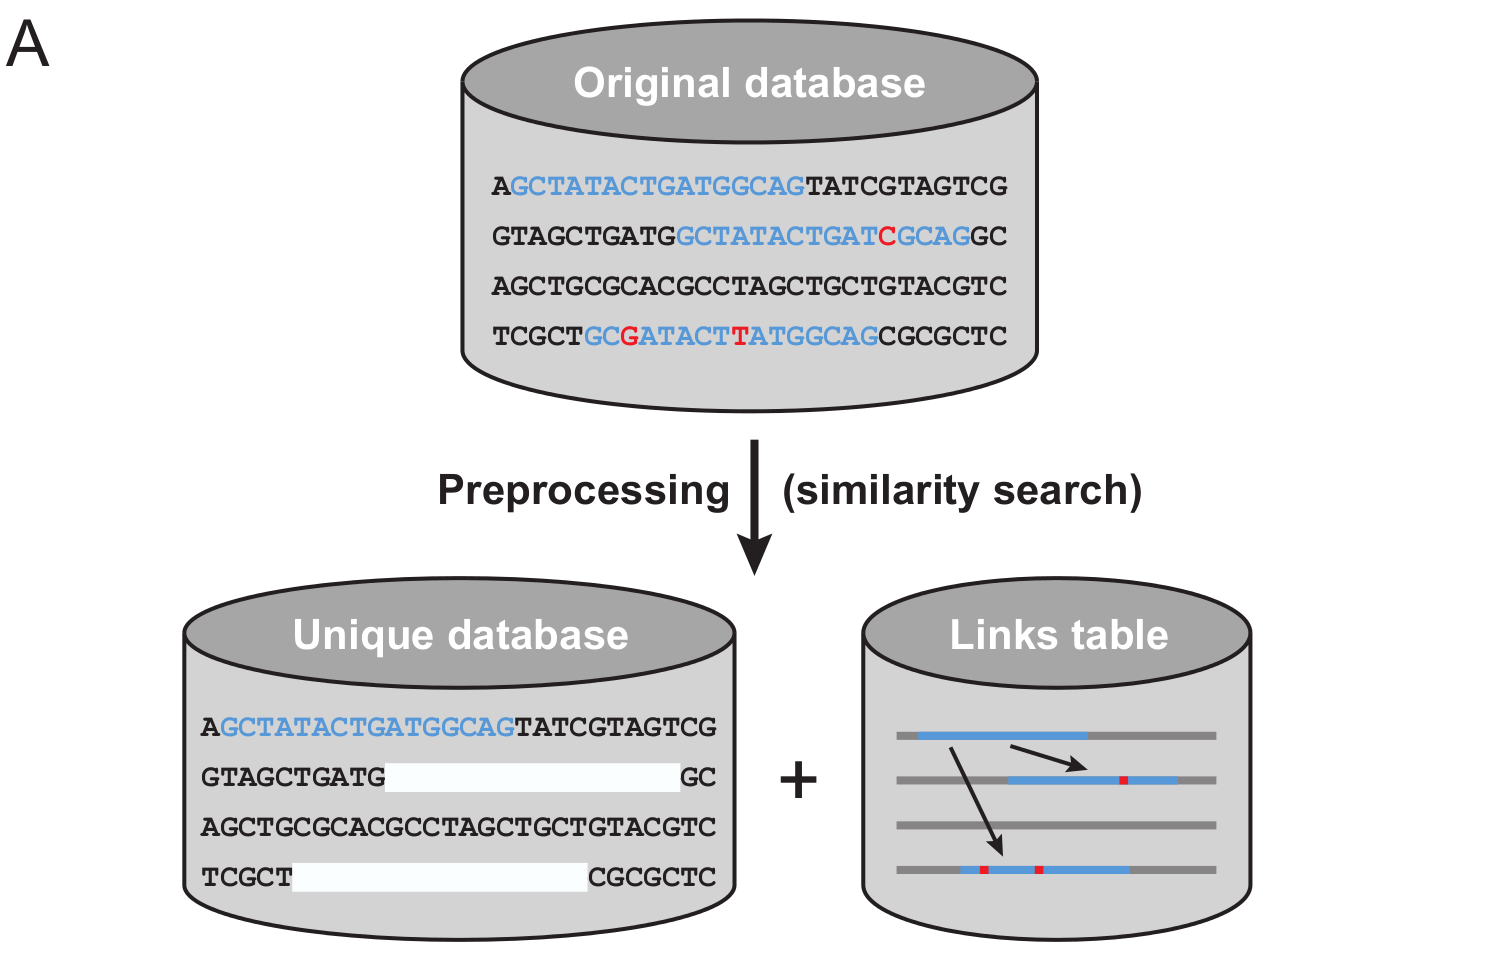
\includegraphics[height=0.3\textwidth]{img/Compgenp1.png}
    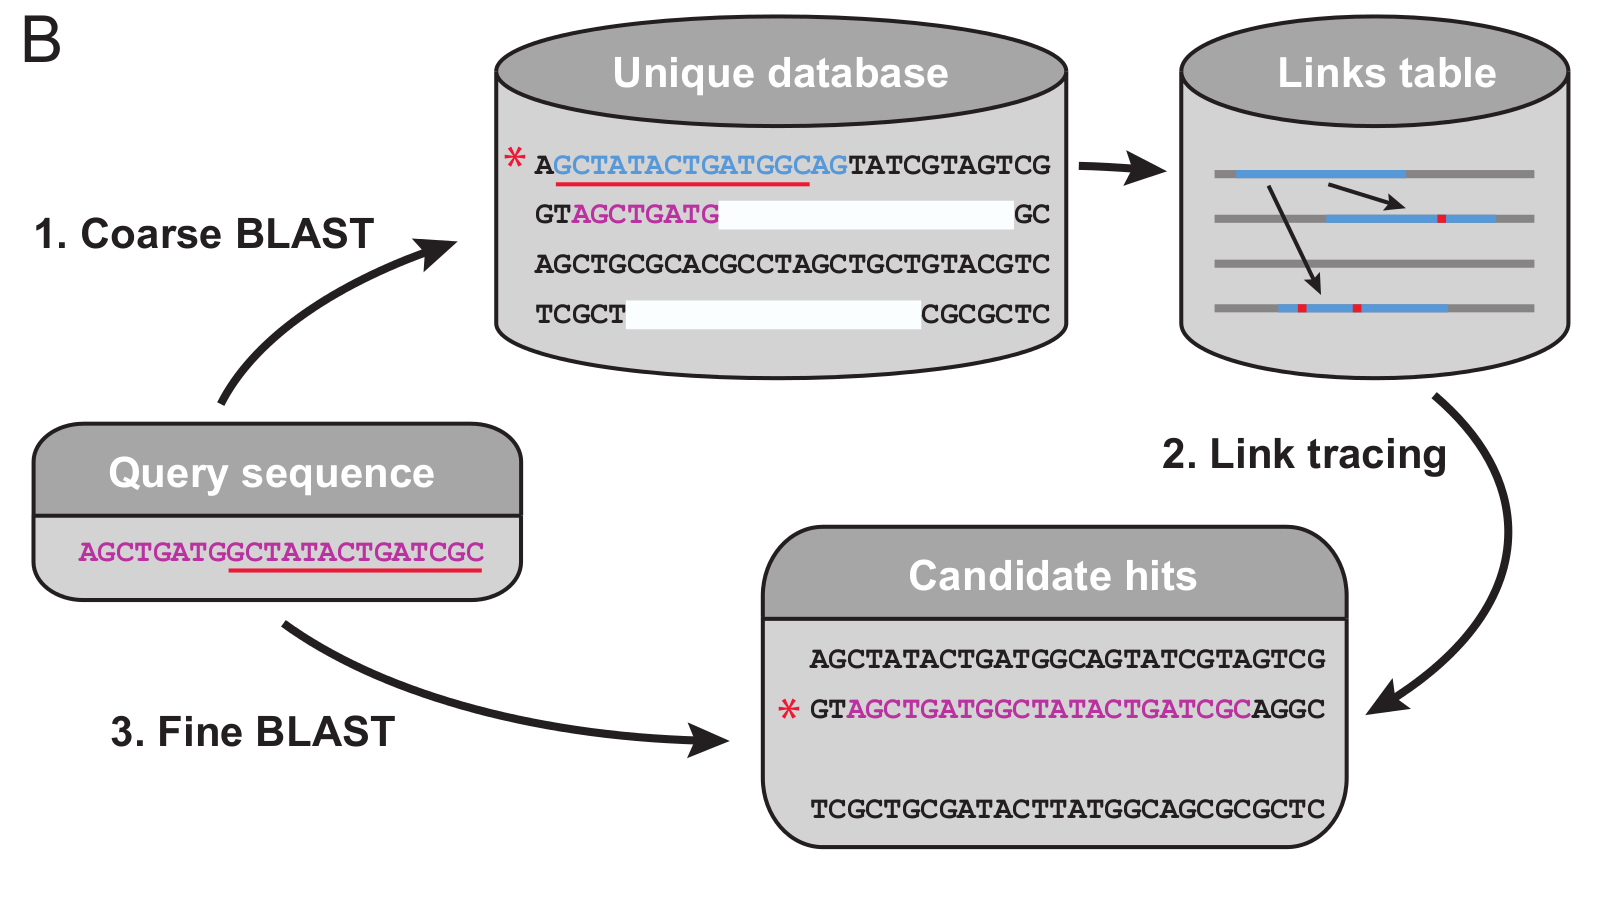
\includegraphics[height=0.3\textwidth]{img/Compgenp2.png}
    %A: Preprocessing: eliminate redundancy
      %for repeats: links in link table to unique database
      %unique db and links table can be shared to parallelize
    %B: Search: 1. blast against unique database with relaxed threshold
    % 2. recover additional candidates via link table
    % 3. BLAST normal against candidate for final result
  \end{figure}
  \end{center}
  %laufzeit preprocessing: linear bis quadratisch, nur einmal nötig
\end{frame}

\begin{frame}{CaBlast - Discussion}
  \begin{itemize}
    \item improved runtime and space requirements
  \end{itemize}
  \begin{center}
    \begin{figure}
      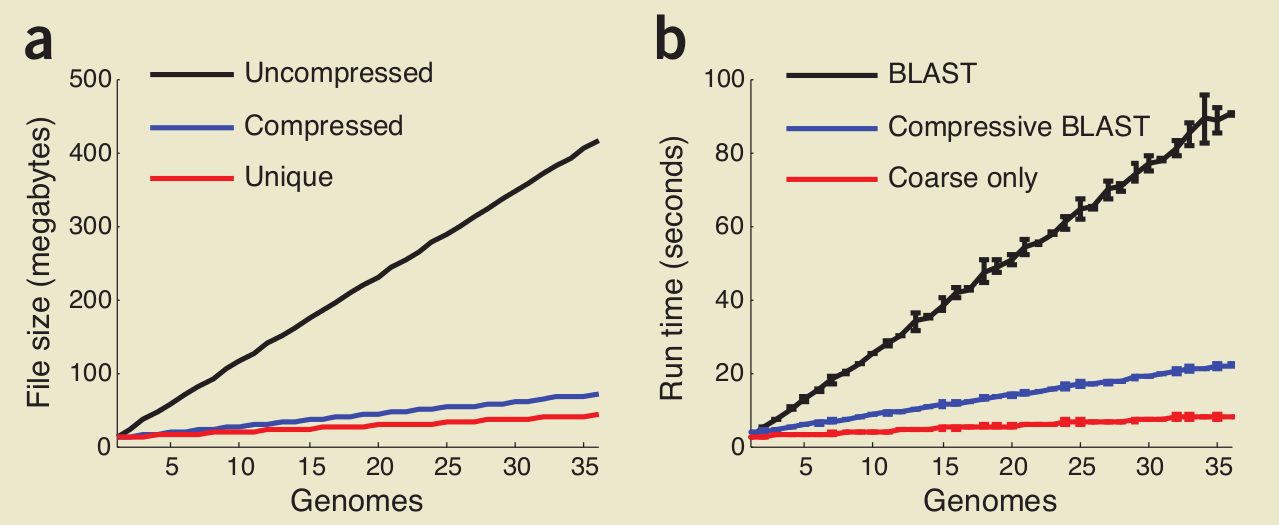
\includegraphics[height=0.3\textwidth]{img/CaBLASTrtfs.png}
    \end{figure}
  \end{center}
\end{frame}

\begin{frame}{Bibliography}
  \begin{itemize}
    \item M. Fritz, R. Leinonen, G. Cochrane, E. Birney: Efficient storage of high throughput DNA sequencing data using 
      reference-based compression, Genome Research, 2011
    \item S. Kuruppu, B. Beresford-Smith, T. Conway, J. Zobel: Iterative Dictionary Construction for Compression of Large
      DNA Datasets, IEEE Transactions on computational Biology and Bioinformatics, 2011
    \item S. Deorowicz, S. Grabowski: Robust Relative Compression of Genomes with Random access, Bioinformatics, 2011, 
      27(21):2979-86
    \item C. Wang, D. Zhang: A novel compression tool for efficient storage of genome resequencing data, Nucleic Acids
      Research, 2011
    \item P. Loh, M.Baym, B. Berger: Compressive Genomics, Nat Biotechnol. 2012, 30(7):627-30
  \end{itemize}
\end{frame}

\end{document}
